\providecommand{\curso}{Séptimo Básico}
\providecommand{\colegio}{Colegio Divina Pastora}
\providecommand{\tituloDocumento}{Guía 3}
\providecommand{\subtituloDocumento}{Tabla de frecuencias (\# 1)}
\providecommand{\tituloItem}{Parte}
\documentclass{cdplf-prueba}
\begin{document}
\subsection{}

Use los datos a continuación para llenar la tabla de frecuencias.

\underline{Datos:} \hspace{4pt} 16 \hspace{4pt}\textbullet\hspace{4pt} 11 \hspace{4pt}\textbullet\hspace{4pt} 15 \hspace{4pt}\textbullet\hspace{4pt} 16 \hspace{4pt}\textbullet\hspace{4pt} 16 \hspace{4pt}\textbullet\hspace{4pt} 16 \hspace{4pt}\textbullet\hspace{4pt} 14 \hspace{4pt}\textbullet\hspace{4pt} 6 \hspace{4pt}\textbullet\hspace{4pt} 11 \hspace{4pt}\textbullet\hspace{4pt} 8 \hspace{4pt}\textbullet\hspace{4pt} 5 \hspace{4pt}\textbullet\hspace{4pt} 7 \hspace{4pt}\textbullet\hspace{4pt} 6 \hspace{4pt}\textbullet\hspace{4pt} 14 \hspace{4pt}\textbullet\hspace{4pt} 4 \hspace{4pt}\textbullet\hspace{4pt} 14 \hspace{4pt}\textbullet\hspace{4pt} 19 \hspace{4pt}\textbullet\hspace{4pt} 10 \hspace{4pt}\textbullet\hspace{4pt} 10 \hspace{4pt}\textbullet\hspace{4pt} 6 \hspace{4pt}\textbullet\hspace{4pt} 18 \hspace{4pt}\textbullet\hspace{4pt} 11 \hspace{4pt}\textbullet\hspace{4pt} 7 \hspace{4pt}\textbullet\hspace{4pt} 4 \hspace{4pt}\textbullet\hspace{4pt} 9 \hspace{4pt}\textbullet\hspace{4pt} 5 \hspace{4pt}\textbullet\hspace{4pt} 10 \hspace{4pt}\textbullet\hspace{4pt} 12 \hspace{4pt}\textbullet\hspace{4pt} 8 \hspace{4pt}\textbullet\hspace{4pt} 13 \hspace{4pt}\textbullet\hspace{4pt} 11 \hspace{4pt}\textbullet\hspace{4pt} 9 \hspace{4pt}\textbullet\hspace{4pt} 12 \hspace{4pt}\textbullet\hspace{4pt} 12 \hspace{4pt}\textbullet\hspace{4pt} 7 \hspace{4pt}\textbullet\hspace{4pt} 16 \hspace{4pt}\textbullet\hspace{4pt} 12 \hspace{4pt}\textbullet\hspace{4pt} 9 \hspace{4pt}\textbullet\hspace{4pt} 10 \hspace{4pt}\textbullet\hspace{4pt} 3 \hspace{4pt}\textbullet\hspace{4pt} 4 \hspace{4pt}\textbullet\hspace{4pt} 7 \hspace{4pt}\textbullet\hspace{4pt} 12 \hspace{4pt}\textbullet\hspace{4pt} 12 \hspace{4pt}\textbullet\hspace{4pt} 3 \hspace{4pt}\textbullet\hspace{4pt} 13 \hspace{4pt}\textbullet\hspace{4pt} 20 \hspace{4pt}\textbullet\hspace{4pt} 5 \hspace{4pt}\textbullet\hspace{4pt} 18 \hspace{4pt}\textbullet\hspace{4pt} 5 \hspace{4pt}\textbullet\hspace{4pt} 13 \hspace{4pt}\textbullet\hspace{4pt} 10 \hspace{4pt}\textbullet\hspace{4pt} 9 \hspace{4pt}\textbullet\hspace{4pt} 16 \hspace{4pt}\textbullet\hspace{4pt} 12
\begin{center}\begin{tblr}{colspec={ccccc},hlines,vlines,hline{2,Z} = {1}{-}{},hline{2,Z} = {2}{-}{},row{even}={black!10},rowsep=0pt}
  .&Frecuencia&Probabilidad&Frecuencia Acumulada&Probabilidad Acumulada \\
 3&&&& \\
 4&&&& \\
 5&&&& \\
 6&&&& \\
 7&&&& \\
 8&&&& \\
 9&&&& \\
 10&&&& \\
 11&&&& \\
 12&&&& \\
 13&&&& \\
 14&&&& \\
 15&&&& \\
 16&&&& \\
 18&&&& \\
 19&&&& \\
 20&&&& \\
 \end{tblr}\end{center}
\subsection{}

Haga un gráfico de barras usando las frecuencias de la tabla anterior.
\begin{center}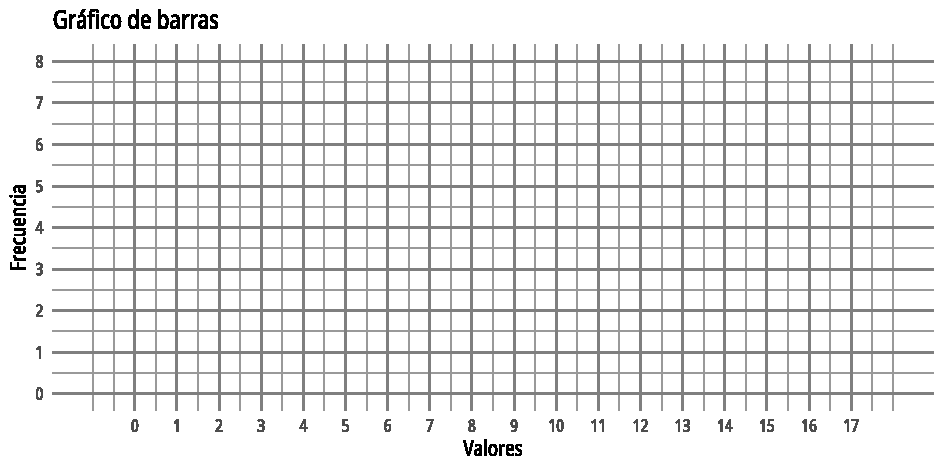
\includegraphics{grafico_vacio_1.pdf}\end{center}

\subsection{}
Usando los resultados anteriores, responda las siguientes preguntas
\begin{tasks}[label={\tcbox[colback=black!60, colframe=black!60, coltext=white, on line, boxsep=0pt, left=3pt, right=3pt, top=2pt, bottom=2pt]{\sffamily\bfseries\alph*}},
item-indent=1.2cm,column-sep=20pt,label-offset=0.3cm,label-width=15pt,after-item-skip=10pt]
    \task! ¿Cuánto vale la media (promedio) de los datos? ¿Qué significa que tenga este valor? \begin{lineas}[height=1.5cm]\end{lineas}
    \task! ¿Cuánto vale la mediana de los datos? ¿Qué significa que tenga este valor? \begin{lineas}[height=1.5cm]\end{lineas}
    \task! ¿Cuál es el rango de los datos? ¿Qué significa que tenga este valor? \begin{lineas}[height=1.5cm]\end{lineas}
    \task! ¿Cuánto vale el primer cuartil de los datos? ¿Qué significa que tenga este valor? \begin{lineas}[height=1.5cm]\end{lineas}
    \task! ¿Cuánto vale el tercer cuartil de los datos? ¿Qué significa que tenga este valor? \begin{lineas}[height=1.5cm]\end{lineas}
    \task! ¿A qué valor corresponde el percentil del 90\%? ¿Qué significa que tenga este valor? \begin{lineas}[height=1.5cm]\end{lineas}
\end{tasks}
\subsection{}

Haga un diagrama de caja usando los datos anteriores.
\begin{center}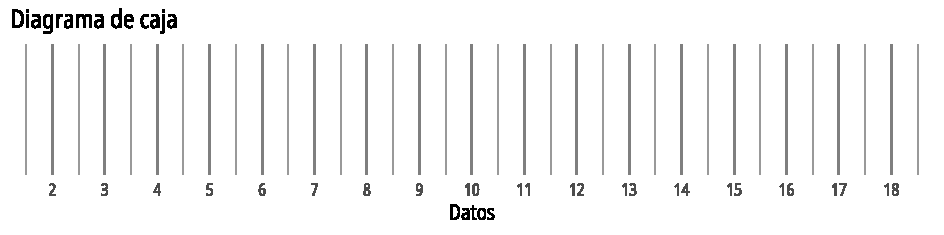
\includegraphics{diagrama_caja_vacio_1.pdf}\end{center}

\newpage\section*{Soluciones}
\setcounter{subsection}{0}
\subsection{}

\begin{center}\begin{tblr}{colspec={ccccc},hlines,vlines,hline{2,Z} = {1}{-}{},hline{2,Z} = {2}{-}{},row{even}={black!10}}
  .&Frecuencia&Probabilidad&Frecuencia Acumulada&Probabilidad Acumulada \\
 3&2&0.036&2&0.036 \\
 4&3&0.055&5&0.091 \\
 5&4&0.073&9&0.164 \\
 6&3&0.055&12&0.219 \\
 7&4&0.073&16&0.292 \\
 8&2&0.036&18&0.328 \\
 9&4&0.073&22&0.401 \\
 10&5&0.091&27&0.492 \\
 11&4&0.073&31&0.565 \\
 12&7&0.127&38&0.692 \\
 13&3&0.055&41&0.747 \\
 14&3&0.055&44&0.802 \\
 15&1&0.018&45&0.82 \\
 16&6&0.109&51&0.929 \\
 18&2&0.036&53&0.965 \\
 19&1&0.018&54&0.983 \\
 20&1&0.018&55&1.001 \\
 \end{tblr}\end{center}
\subsection{}
\begin{center}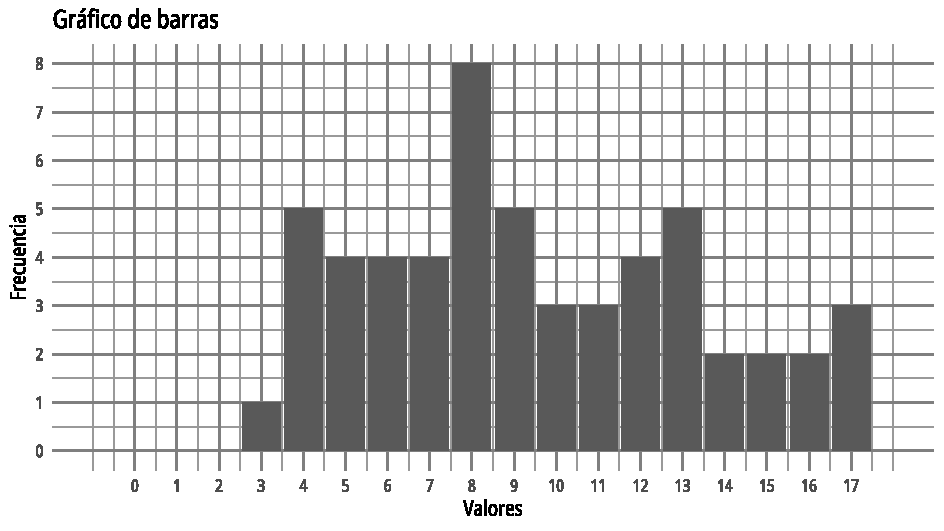
\includegraphics{grafico_barras_1.pdf}\end{center}
\subsection{}
\begin{tasks}[label={\tcbox[colback=black!60, colframe=black!60, coltext=white, on line, boxsep=0pt, left=3pt, right=3pt, top=2pt, bottom=2pt]{\sffamily\bfseries\alph*}},
item-indent=1.2cm,column-sep=20pt,label-offset=0.3cm,label-width=15pt,after-item-skip=10pt,item-format=\raggedright](2)\task La media es 10.564.
 Esto significa que los valores más frecuentes son los que están cercanos a 10.564, y es donde también se encuentran las barras más altas 
 en el gráfico de barras.\task La mediana es 11. 
 Esto significa que la mitad (50\%) de los datos tiene un valor menor 
 o igual a 11.\task El rango de los datos es 17. Esto 
 significa que la distancia entre el máximo (20) y el mínimo (3) de los datos es 17.\task El primer cuartil es 7. Esto significa que un cuarto de los datos (25\%) tiene un valor 
 menor o igual a 7.\task El tercer cuartil es 14. Esto significa que tres cuartos de los datos (75\%) tiene un valor menor
 o igual a 14.\task El percentil del 90\% es 16. Esto significa que el 90\% de los datos tiene un valor menor o igual a 16.\end{tasks}
\subsection{}
\begin{center}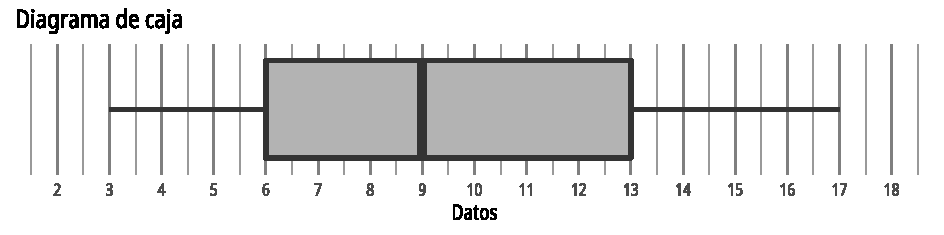
\includegraphics{diagrama_caja_1.pdf}\end{center}
\end{document}
